% Source-derived chapter 15: Surfaces  with restricted configurations
% Original source: no-enriques-surface-over-the-integers
\chapter{Surfaces  with restricted configurations}
\label{no-enriques-surface-over-the-integers-chapter-15}
\source{no-enriques-surface-over-the-integers}

\begin{remark}[Source section]
\label{no-enriques-surface-over-the-integers-chapter-15-source}
\source{no-enriques-surface-over-the-integers}
\source{no-enriques-surface-over-the-integers}
This chapter reproduces the corresponding section of the retrieved
LaTeX source, including its definitions, statements, examples, and
proofs. It has not yet been translated into Lean.
\notready
\end{remark}

% The source section title was: Surfaces  with restricted configurations
\mylabel{Restricted configurations}

Let $k$ be an algebraically closed ground field $k$ of arbitrary characteristic $p\geq 0$,
and $Y$ be a classical Enriques surface. The goal of this section is
to show that certain configurations of $(-2)$-curves cannot exist, once one imposes rather severe 
restrictions on the configuration of reducible fibers in genus-one fibrations.

\begin{proposition}
\source{no-enriques-surface-over-the-integers}
\notready
\mylabel{only two configurations}
There is no classical Enriques surface $Y$ such that every genus-one fibration $\varphi:Y\ra\PP^1$
satisfies one of the following properties:
\begin{enumerate}
\item
The configuration of reducible fibers is $\I_1^*+\I_4$, where the $\I_1^*$-fiber is multiple.
\item
The configuration  is $\I_2^*+\III+\III$, where two of these fibers are multiple.
\end{enumerate}
\end{proposition}

\proof 
Seeking a contradiction, we assume that such a surface exists. Choose a genus-one fibration $\varphi:Y\ra \PP^1$.
By \cite{Ekedahl; Shepherd-Barron 2004}, Theorem A the surface $Y$ is non-exceptional.
According to Proposition \ref{properties non-exceptional} there is another genus-one fibration $\psi:Y\ra\PP^1$,
with $\varphi^\inv(\infty)\cdot\psi^\inv(\infty)=4$. Choose a multiple fiber  $2F\subset Y$ for   $\psi$.
Without restriction, we may assume that the fibers of $\varphi$ and $\psi$ with Kodaira symbol $\I_n^*$ occur over
$t=\infty$. 

Suppose first that $\varphi^\inv(\infty)$ has Kodaira symbol $\I_1^*$, and hence must be multiple. The dual graph is:
\begin{equation*}
% dual graph I1*
\begin{gathered}
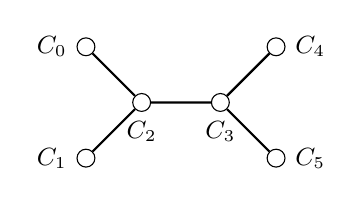
\begin{tikzpicture}
[node distance=1cm, font=\small]
\tikzstyle{vertex}=[circle, draw, fill=white, inner sep=0mm, minimum size=1.5ex]
\node[vertex]	(C2)  	at (1,0) [			label=below:{$C_2$}]	{};
\node[vertex]	(C3)	[right of=C2, 		label=below:{$C_3$}]	{};
\node[vertex]	(C4)	[above right of=C3, label=right:{$C_4$}]	{};
\node[vertex]	(C5)	[below right of=C3, label=right:{$C_5$}]	{};
\node[vertex]	(C0)	[above left of=C2, 	label=left :{$C_0$}]	{};
\node[vertex]	(C1)	[below left of=C2, 	label=left :{$C_1$}]	{};
 
\draw [thick] (C2)--(C3)--(C4);
\draw [thick] (C0)--(C2)--(C1);
\draw [thick] (C5)--(C3)--(C4);
\end{tikzpicture}
\end{gathered}
\end{equation*}
After renumeration, we may assume $(F\cdot C_0)=1$. The curve $C_1+\ldots +C_5$ has dual graph 
$T_{2,2,3}$ and is $\psi$-vertical, hence must belong to $\psi^\inv(\infty)$. Suppose the latter has Kodaira symbol
$\I_1^*$. Then $\psi^{-1}_\red(\infty)=R+C_1+\ldots+C_5$ for some additional component 
$R$ with $(R\cdot C_2)=1$, and the fiber is multiple. This gives the contradiction
$$
1=\varphi^\inv_\ind(\infty)\cdot\psi^\inv_\ind(\infty) = (C_0+2C_2)\cdot R = (C_0\cdot R) + 2\geq 2.
$$
Thus $\psi^\inv(\infty)$ has Kodaira symbol $\I_2^*$, and we write $\psi^\inv_\ind(\infty)=R+R'+C_1+\ldots+C_5$
with additional components $R$ and $R'$, which have  $(R\cdot C_1)=(R'\cdot C_1)=1$. Then
$$
2\geq \varphi^\inv_\ind(\infty)\cdot\psi^\inv_\ind(\infty) = (C_0+C_1)\cdot (R+R') = C_0\cdot(R+R')  + 1+1.
$$
Hence $R\cup R'$ is disjoint from $C_0$, and $\psi^\inv(\infty)$ must be simple. 
Without restriction, we may assume that $\psi^\inv(0)$ is multiple with Kodaira symbol $\III$.
Write $\psi^\inv_\ind(0)=D+D'$. Then
$$
2(D+D')\cdot C_0=\psi^\inv(\infty)\cdot C_0 =2C_2\cdot C_0 = 2.
$$
Without restriction, we may assume $(C_0\cdot D)=1$ and $(C_0\cdot D')=0$.
Then the dual graph for our curves becomes:
\begin{equation*}
% dual graph I1*
\begin{gathered}
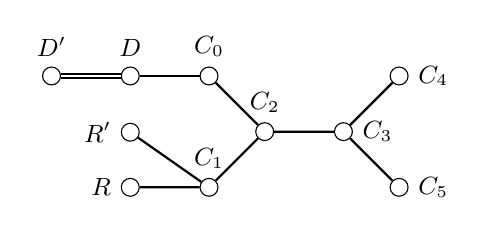
\begin{tikzpicture}
[node distance=1cm, font=\small]
\tikzstyle{vertex}=[circle, draw, fill=white, inner sep=0mm, minimum size=1.5ex]
\node[vertex]	(C2)  	at (1,0)	[		label=above:{$C_2$}]	{};
\node[vertex]	(C3)	[right of=C2, 		label=right:{$C_3$}]	{};
\node[vertex]	(C4)	[above right of=C3, label=right:{$C_4$}]	{};
\node[vertex]	(C5)	[below right of=C3, label=right:{$C_5$}]	{};
\node[vertex]	(C0)	[above left of=C2, 	label=above:{$C_0$}]	{};
\node[vertex]	(C1)	[below left of=C2, 	label=above   :{$C_1$}]	{};
 
\node[vertex]	(R)	[left of=C1, 		label=left:{$R$}]	{};
\node[vertex]	(R')	[above  of=R, yshift=-.3cm,	label=left:{$R'$}]	{};
\node[vertex]	(D)	[left of=C0, 		label=above:{$D$}]	{};
\node[vertex]	(D')	[left of=D, 		label=above:{$D'$}]	{};

\draw [thick] (C2)--(C3)--(C4);
\draw [thick] (C0)--(C2)--(C1);
\draw [thick] (C5)--(C3)--(C4);
\draw [thick] (C0)--(D);
\draw [thick, double] (D')--(D);

\draw [thick] (R)--(C1)--(R');

\end{tikzpicture}
\end{gathered}
\end{equation*}
Thus $R+D+C_0+\ldots+C_4$ is a curve of canonical type $\IV^*$, contradiction.

\emph{ Summing up, every  genus-one fibration on $Y$ 
 has   $\I_2^*+\III+\III$ as configuration of degenerate fibers, two of which are multiple.}
We tacitly assume that  the $\I_2^*$-fiber lies over $t=\infty$, whereas the
$\III$-fibers appear over $t=0,1$. 
In particular,  the  dual graph for the reducible fibers of our $\varphi:Y\ra\PP^1$ is:
\begin{equation*}
% dual graph I2*+III+III
\begin{gathered}
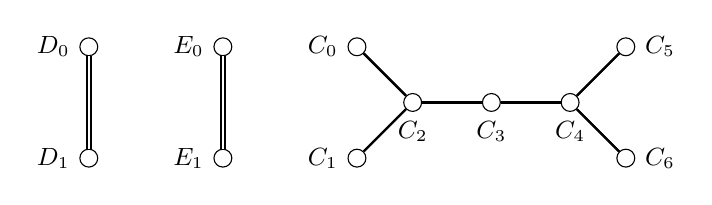
\begin{tikzpicture}
[node distance=1cm, font=\small]
\tikzstyle{vertex}=[circle, draw, fill=white, inner sep=0mm, minimum size=1.5ex]
\node[vertex]	(C2)  	at (1,0) [			label=below:{$C_2$}]	{};
\node[vertex]	(C3)	[right of=C2, 		label=below:{$C_3$}]	{};
\node[vertex]	(C4)	[right of=C3, 		label=below:{$C_4$}]	{};
\node[vertex]	(C5)	[above right of=C4, label=right:{$C_5$}]	{};
\node[vertex]	(C6)	[below right of=C4, label=right:{$C_6$}]	{};
\node[vertex]	(C0)	[above left of=C2, 	label=left :{$C_0$}]	{};
\node[vertex]	(C1)	[below left of=C2, 	label=left :{$C_1$}]	{};

\node[vertex]	(E0)			[left  of=C0, xshift=-2em, label=left :{$E_0$}]	{};
\node[vertex]	(E1)			[left  of=C1, xshift=-2em, label=left :{$E_1$}]	{};
\node[vertex]	(D0)			[left  of=E0, xshift=-2em, label=left :{$D_0$}]	{};
\node[vertex]	(D1)			[left  of=E1, xshift=-2em, label=left :{$D_1$}]	{};


\draw [thick] (C2)--(C3)--(C4);
\draw [thick] (C0)--(C2)--(C1);
\draw [thick] (C6)--(C4)--(C5);
\draw [thick,double] (D0)--(D1);
\draw [thick,double] (E0)--(E1);

\draw [thick] (C2)--(C3)--(C4);
\draw [thick] (C0)--(C2)--(C1);
\draw [thick] (C6)--(C4)--(C5);
\end{tikzpicture}
\end{gathered}
\end{equation*}
We first verify that $\varphi^{-1}(\infty)$ is simple. Seeking a contradiction, we assume that it is multiple,
such that $F\cdot \varphi^{-1}_\ind(\infty)=1$. After renumeration  we may assume $(F\cdot C_0)=1$.
The connected curve $C_1+\ldots+C_6$ has dual graph $T_{2,2,4}$, hence is contained in $\psi^{-1}(\infty)$.
Let $R\subset\psi^{-1}(\infty)$ be the additional component, which has $(R\cdot C_2)=1$.
From
$$
2\geq \varphi^{-1}_\ind(\infty)\cdot \psi^{-1}_\ind(\infty) = (C_0+2C_2)\cdot R = (C_0\cdot R) + 2
$$
we infer $R\cap C_0=\varnothing$. Thus $C_0+\ldots +C_3+R$ supports a curve of canonical type $\I_0^*$, 
contradiction.

\emph{Summing up, in  all genus-one fibrations the $\I_2^*$-fiber   is simple and the $\III$-fibers  
are multiple.} Recall that $2F$ is a multiple fiber for our fibration $\psi:Y\ra\PP^1$ with $\varphi^\inv(\infty)\cdot\psi^\inv(\infty)=4$.
After renumeration, we may assume that $(F\cdot D_0)=(F\cdot E_0)=1$ and $(F\cdot D_1)=(F\cdot E_1)=0$.
In particular, the curves $D_0$, $E_0$ are $\psi$-horizontal, whereas $D_1$, $E_1$ are $\psi$-vertical.

By symmetry, we now write  $\psi^{-1}_\ind(0)=R_0+R_1$ such that $R_0$ is $\varphi$-horizontal and  $R_1$ is $\varphi$-vertical.
We claim that $R_1$ is not contained in $\varphi^{-1}(0)$. 
For $R_1=D_1$ we get the contradiction
$$
1=(D_0+D_1)\cdot (R_0+R_1) = D_0\cdot (R_0+R_1)\geq (D_0\cdot R_1)=(D_0\cdot D_1)=2,
$$
whereas $R_1=D_0$ leads to  
$$
1=(D_0+D_1)\cdot (R_0+R_1) = D_1\cdot(R_0+R_1)    = 0,
$$
again a contradiction. Thus $R_1$ is disjoint from $\varphi^{-1}(0)$, which gives 
$$
(D_0\cdot R_0) = D_0\cdot (R_0+R_1) = (D_0+D_1)\cdot (R_0+R_1) = 1.
$$
By symmetry, we also get $(E_0\cdot R_0)=1$.
Likewise, we write $\psi^\inv_\ind(1)=S_0+S_1$ such that $S_0$ is $\varphi$-horizontal and  $S_1$ is $\varphi$-vertical,
and see $(D_0\cdot S_0)=(E_0\cdot S_0)=1$.
Thus   $D_0+ R_0+E_0+S_0$ is a curve of canonical type $\I_4$, contradiction.
\qed


%===========================================================
